\documentclass[10pt,aspectratio=169]{beamer}

\usepackage[english]{babel}
\usepackage{t1enc}
\usepackage{pgfpages}
\usepackage{array}

\usetheme{default}
\setbeamercovered{transparent}
\setbeamertemplate{navigation symbols}{}
\setbeamertemplate{footline}{
\usebeamercolor[fg]{title}%
\hfill\insertframenumber{}/\inserttotalframenumber \phantom{xx}
}

\usepackage{enumitem}
\setlist[itemize]{label=\textcolor{blue}{$\bullet$}}


\newcommand{\blue}{\color{blue}}
\newcommand{\red}{\color{red}}
\newcommand{\black}{\color{black}}
\newcommand{\darkred}{\color{darkred}}
\newcommand{\darkgreen}{\color{darkgreen}}

\begin{document}
\section{Toolchains, \texttt{mk}, libraries and header files}
\title{Shared Libraries}
\author{Paolo Joseph Baioni\\ \href{mailto:paolojoseph.baioni@polimi.it}{\color{blue}paolojoseph.baioni@polimi.it}}
\date{\today}

\begin{frame}
  \maketitle
\end{frame}

\begin{frame}{Toolchains}
    A \textbf{toolchain} is a set of software which constitutes a closed environment for the development of further software.
    The toolchain encapsulates:
  \begin{itemize}
      \item a compiler (and related standard library)
  \item a linker
  \item basic tools for software development
  \item basic libraries for scientific development
  \end{itemize}	

    The software \textbf{must} be independent from the hosting OS.

    \vfill
    \textbf{Example} The {\ttfamily mk} toolchains you find (containerised) in {\ttfamily /software} on the cluster.
\end{frame}

\begin{frame}{How do I confine my work inside a specific toolchain?}

    The \texttt{Bash} environment variables define paths for executables and libraries; the tool to manage these variables is commonly called the \textbf{environment module system}.

  There are two main module systems, one is named \texttt{Lmod} and the other is \texttt{TCL Environment Modules}.\\[3mm]

    A \textbf{module} is basically a set of instructions that define a specific environment for a specific software: where are the \textit{executables}, where are its \textit{libraries}, where are the \textit{header files}, $\dots$

    {If the software is built inside a toolchain, the installation and the environment  will be portable.} \\[3mm]

A specific module is “loaded” and can be “unloaded” as well when not needed.
The module system can define a hierarchy: a module may need another one, and the system automatically handles these dependencies.

    \vfill
    \textbf{Remark} {\ttfamily Spack} provides a similar functionality via {\ttfamily spack load}, and can build modulefiles for you, as we'll see in the next lab.
\end{frame}


\begin{frame}[fragile]{How to use a third-party library}
  Basic compile/link flags:
\begin{verbatim}
$ g++ -I${mkLibrarynameInc} -c main.cpp
$ g++ -L${mkLibrarynameLib} -llibraryname main.o -o main
\end{verbatim}
\bigskip
\textbf{Warning}: by mistake, one can include headers and link against libraries related to different installations/versions of the same library! The compile, link and loading phase may succeed, but the executable may crash, resulting in a very subtle yet painful error to debug!
\end{frame}

\begin{frame}{Using shared libraries}
   Shared libraries:
   \begin{itemize}
       \item User point of view
       \item Developer point of view
   \end{itemize}

  \medskip
   Users need to take care to 
   \begin{itemize}
       \item \textbf{linking} phase during compilation
       \item \textbf{loading} phase at execute time
   \end{itemize}

  \medskip
   Developers usually contribute to a
   \begin{itemize}
       \item \textbf{development} phase
       \item \textbf{release} phase
   \end{itemize}

\end{frame}


\begin{frame}{Versions and releases} 
  The \emph{version} is a symbol
  (typically a number) by which we indicate a set of instances of a
  library with a common public interface and functionality.
  \smallskip

    Within a version, one may have several \textit{releases}, typically indicated
  by one or more numbers (major and minor or bug-fix). A new release is 
  issued to fix bugs or improve a library without
  changes in its public interface. So a code linked against version 1,
  release 1 of a library should work (in principle) when you update
  the library to version 1, release 2.
  \smallskip

  Normally versions and releases are separated by a dot in the library name:
  \texttt{libfftw3.so.3.3.9} is version 3, release 3.9 of the
  \texttt{fftw3} library (The Fastest Fourier Transform in the West).

  \begin{center}
      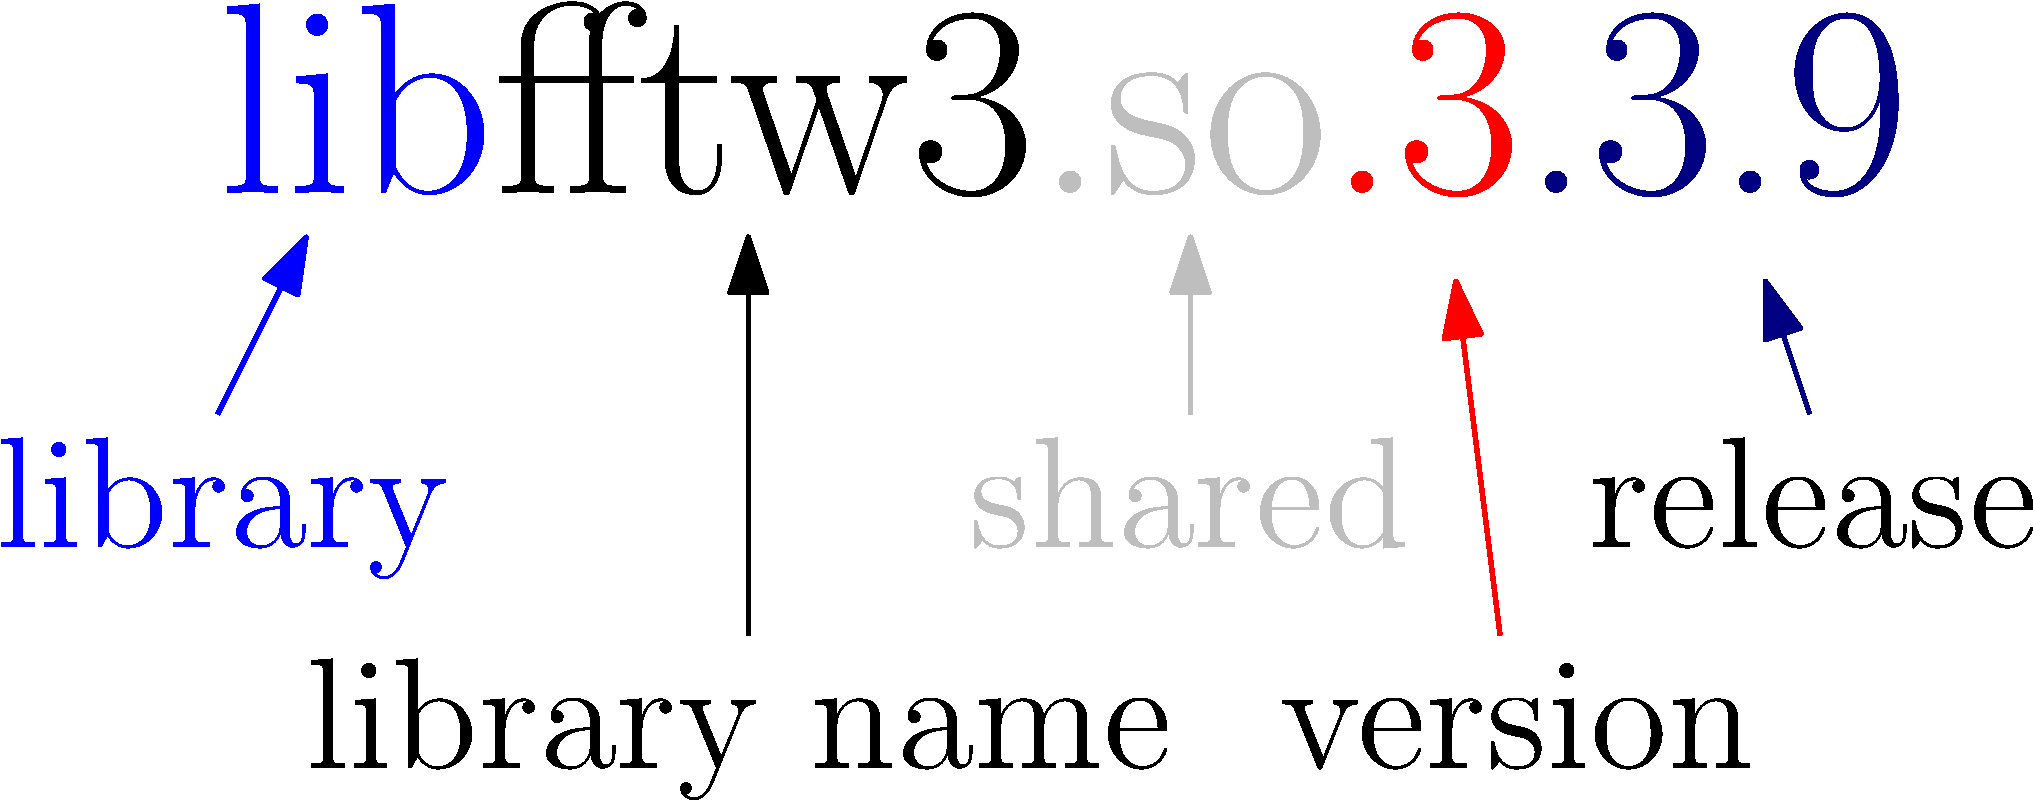
\includegraphics[width=0.45\textwidth]{ipe/libExplained.pdf}
  \end{center}

\end{frame}

\begin{frame}[fragile]{Naming scheme of shared libraries (Linux/Unix)}
  We give some nomenclature used when describing a shared library

  \begin{itemize}
      \item \textbf{link name}: name used in the linking stage when
    you use the \texttt{-lmylib} option.  
    \item \textbf{soname}: \textit{shared object name} looked for
    by the \emph{loader} stage.  
\item \textbf{full name}: name of the actual file that stores the library. 
  \end{itemize}
\medskip

    Example:
    \begin{itemize}
        \item[] \texttt{fftw}: is the \textit{link name}.
        \item[] \texttt{libfftw3.so.3}: is the \textit{soname}.
        \item[] \texttt{libfftw3.so.3.3.9}: is the \textit{real name} of the file.
    \end{itemize}

    We call a \textit{fully qualified library} a soname that contains the full path to the library.
\end{frame}


\begin{frame}[fragile]{How does it work?}  The command
  \texttt{ldd} lists the shared libraries used by an object file. \\
  \medskip
  
\textbf{Example:}
\begin{verbatim}
$ ldd ${mkOctavePrefix}/lib/octave/6.2.0/liboctave.so
...
libfftw3.so.3 =>
     /u/sw/toolchains/gcc-glibc/11.2.0/pkgs/fftw/3.3.9/lib/libfftw3.so.3
...
\end{verbatim}
\begin{itemize}
	\item \texttt{Octave} has been linked to \texttt{libfftw3}.
\end{itemize}

The \textbf{loader} searches for this library, finding its fully qualified name. \\ \medskip

\textbf{Which release?} 
\begin{verbatim}
$ ls -l ${mkFftwLib}/libfftw3.so.3
/full/path/to/libfftw3.so.3 -> libfftw3.so.3.3.9
\end{verbatim}
I am in fact using release \texttt{3.9} of version \texttt{3}.
\end{frame}

\begin{frame}{Explanation}  

  The executable (\texttt{octave}) contains the
  information on which shared library to load, including version
  information (its \texttt{soname}). This part has been taken care of by the 
  developers of \texttt{Octave}.
  \smallskip

  When I launch the program the loader looks in special directories,
  among which \texttt{/usr/lib} for a file that matches the
  \texttt{soname}. This file is typically a symbolic link to the real
  file containing the library.  
  \medskip

  If I have a new release of \texttt{fftw3} version 3, let's say $3.4.1$,
  I just need to place the corresponding shared library file, reset the symbolic links and automagically \texttt{octave}
  will use the new release (this is what \texttt{apt} does when
  installing a new update in a Debian/Ubuntu system, for example).

  \smallskip

  No need to recompile anything!
\end{frame}


\begin{frame}[fragile]{Another nice thing about shared libraries} 

  A shared library may depend on another shared library. This information may be encoded  when creating the library
  (just as for an executable, we will see it later on).

  For instance
\begin{verbatim}
$ ldd /usr/lib/x86_64-linux-gnu/libumfpack.so.5
...
libblas.so.3 => /lib/x86_64-linux-gnu/libblas.so.3
...
\end{verbatim}
The UMFPACK library is linked against version
\texttt{3} of the BLAS library. \smallskip

This prevents using incorrect version of
libraries. Moreover, when creating an executable that needs UMFPACK I only have to indicate
\texttt{-lumfpack}! \\
\textbf{Note}: This is not true for static libraries: you have to list all dependencies.
\end{frame}

\begin{frame}[fragile]{How to link against a shared library}   
  It is now sufficient to proceed as usual
\begin{verbatim}
g++ -I${mkFFtwInc} -c main.cpp
g++ -L${mkFFtwLib} -lfftw3 main.o -o main
\end{verbatim}

The linker finds \texttt{libfftw3.so}, controls the symbols it
provides and verifies if the library contains a
\texttt{soname} (if not the link name is assumed to be also the
soname).

Indeed \texttt{libfftw3.so} provides a \texttt{soname}. If we wish we
can check it:
\begin{verbatim}
$ objdump libx.so.1.3 -p | grep SONAME
SONAME   libfftw3.so.3
\end{verbatim}
(of course this has been taken care by the library developers).
\end{frame}

\begin{frame}[fragile]

  Being \texttt{libfftw3.so} a shared library the linker does not
  resolve the symbols by integrating the corresponding code in the
  executable. Instead, it inserts the information about the
  \texttt{soname} of the library:
  \smallskip

\begin{verbatim}
$ ldd main
libfftw3.so.3 => /full/path/to/libfftw3.so.3
\end{verbatim}
\smallskip
The loader can then do its job now!
\smallskip

In conclusion, linking with a shared library is not more complicated
than linking with a static one.
\medskip

\textbf{Remember:} By default if the linker finds both the static and
shared version of a library it gives precedence to the shared
one. If you want to be sure to link with the static version you need to use 
the \texttt{-static} linker option.
\end{frame}

\begin{frame}{Directories where the loader searches the shared libraries}  
	
	\begin{itemize}
		\item  \texttt{/lib*} or  \texttt{/usr/lib*} .
		\item Additional directories can be specified by \texttt{/etc/ld.so.conf} and files inside the directory \texttt{/etc/ld.so.conf.d/}.
	\end{itemize}


  The command \texttt{ldconfig} rebuilds the database of the shared
  libraries and should be called every time one adds a new library (of
  course \texttt{apt} does it for you, and moreover
  \texttt{ldconfig} is launched at every boot of the computer).
  \smallskip

  \textbf{Note}: all these operations require you to act as superuser, for
  instance with the \texttt{sudo} command.
\end{frame}

\begin{frame}[fragile]{Alternative ways of directing the loader}
  \begin{itemize}
  \item Setting the environment variable \texttt{LD\_LIBRARY\_PATH}. If
    it contains a colon-separated list of directory names the
    loader will first look for libraries on these directories (analogous to \texttt{PATH} for executables):
\begin{verbatim}
  export LD_LIBRARY_PATH+=:dir1:dir2
\end{verbatim}
\item With the special flag \texttt{-Wl,-rpath=directory}
  during the compilation of the executable, for instance
\begin{verbatim}
  g++ main.cpp -o main -Wl,-rpath=/opt/lib  -L. -lsmall
\end{verbatim}
Here the loader will look in \texttt{/opt/lib} before the standard directories. You can also use relative paths. See e.g. \href{https://gcc.gnu.org/onlinedocs/gcc/Directory-Options.html}{\color{blue}gcc directory options} and \href{https://gcc.gnu.org/onlinedocs/gcc/Link-Options.html}{\color{blue}gcc link options}
\item Launching the command \texttt{sudo ldconfig -n directory} which adds \texttt{directory} to the loader search path (superuser privileges are required). This addition remains valid until the next reboot of the computer. \textbf{Note}: \underline{prefer the other alternatives!}
  \end{itemize}
\end{frame}

\begin{frame}[fragile]{How to build a shared library?}
  We will dedicate exercise 1 to this issue, where we will also show how to handle shared libraries and symbols dynamically.
  We need to know only the following:
  \begin{itemize}
  \item When building a shared library we need to pass the option \texttt{-shared} to the linker
  \item Object code used in a shared library must be \emph{position independent} (compiler option \texttt{-fPIC})
  \end{itemize}

  Basic build of a shared library starting from an object file:
\begin{verbatim}
$ g++ -shared -Wl,-soname,libutility.so utility.o -o libutility.so
\end{verbatim}
\end{frame}

\section*{Exercises}

\begin{frame}
\centering
{\usebeamercolor[fg]{structure} \huge Exercises}\\

\vspace{1cm}

\large Paolo Joseph Baioni \\ \href{mailto:paolojoseph.baioni@polimi.it}{\normalsize\color{blue}paolojoseph.baioni@polimi.it}\\

\vfill\today
\end{frame}

\begin{frame}{Exercise 1: quadrature rules with plugins}
\begin{itemize}
\item Implement a code that enables the user to compute the integral of a scalar function by selecting the quadrature rule as the name of a dynamically loadable object;
\item The dynamically loadable object should define a function with the following signature:
\texttt{double integrate(std::function<double (double)>, double a, double b)}.
\item Implement plugins for midpoint and trapezoidal rule.
\item {\color{gray}Implement a plugin for quadrature with adaptive refinement.}
\end{itemize}
\end{frame}

\begin{frame}{Exercise 2: 1D interpolator using generic programming}
This exercise (inspired by \texttt{Examples/src/Interp1D}) shows how to use policies, taking as example a generic piecewise linear 1D interpolator, with an application to
vectors of pairs of values (representing the interpolation nodes and the corresponding values) and to two separate vectors (one for the nodes and one for the values).

It is rather generic and accepts as an input iterators to any container with bi-directional iterators. Bi-directionality is indeed only needed for extrapolation on the right.
\end{frame}

\section{Makefiles}
\begin{frame}
\centering
{\usebeamercolor[fg]{structure} \huge Useful recalls on Make and Makefiles}\\

\vspace{1cm}

\large Paolo Joseph Baioni \\ \href{mailto:paolojoseph.baioni@polimi.it}{\normalsize\color{blue}paolojoseph.baioni@polimi.it}\\

\vfill\today
\end{frame}

\begin{frame}{Main variables for implicit rules}
\begin{tabular}{>{\ttfamily}l|l} CXX & the c++ compiler (g++)\\
  CPPFLAGS & Options for the C preprocessor\\
  CXXFLAGS & Options for the
             C++ compiler\\
  CCFLAGS & Options for the C compiler\\
  FFLAGS & Options for the Fortran compiler\\
  LDFLAGS & Options for the linker \alert{(not for indicating libraries!)}\\   LDLIBS & To indicate libraries to be loaded\\
  LINK.o & The command used for the linking stage\\
  TARGET\_ARCH & The target architecture\\
\end{tabular}
\medskip

The macro \alert{LINK.o} is the command for calling the {\blue linker}
on object files \texttt{*.o}. By default it is equal to \texttt{cc}, i.e. it uses the C linker as linker. If you are using C++ it's better to change it so that it loads the standard library, by setting
\begin{semiverbatim}
    LINK.o = \$(CXX) \$(LDFLAGS) \$(TARGET\_ARCH)
\end{semiverbatim}

\smallskip
\end{frame}

\begin{frame}{Other useful implicit variables}

  \begin{tabular}{>{\ttfamily}l|l}
RM & Command to remove files (rm -f)\\
CC & The C compiler (gcc)\\
    FC & The Fortran compiler (gfortran)\\
    CPP & The C preprocessor (\$(CC) -E)\\
    AR  & The command to produce static library (ar)\\
    ARFLAGS & The flags for AR (rv)
\end{tabular}
\end{frame}

\begin{frame}
  \frametitle{Common Preprocessor options in \texttt{CPPFLAGS}}
 \hspace*{-0.5cm}
  \begin{tabular}{>{\ttfamily}l|p{7.6truecm}}
    -I<dirname> & Add <dirname> to the directories to search for included (header) files\\
    -D<Macro> & Define pre-processor variable <Macro>\\
    -D<Macro=value> & Provide value to pre-processor variable <Macro>\\
    -DNDEBUG & Activate the \texttt{NDEBUG} cpp variable, used
               to indicate that the code should be optimized.
  \end{tabular}  
\end{frame}

\begin{frame}
  \frametitle{Common c++ compiler options in \texttt{CXXFLAGS}}
 \hspace*{-0.5cm}
  \begin{tabular}{>{\ttfamily}l|p{7.6truecm}}
    -g & Activate debugging (it implies \texttt{=O0})\\
    -O[0-3]& Optimization level (0 none, 3 maximal)\\
    -Og & Perform only optimizations that allow reasonable debugging\\
    -Ofast & Perform also optimizations that don't comply with IEEE standard
    (implies -O3)\\
    -fPIC &  Generate position-independent code suitable for use in a
            shared library\\
    -fpic & Another version of \texttt{-fPIC}\\
    -std=[standard] & Use a specific standard. Possible
                      \texttt{[standard]} may be
                      \texttt{c++11} or \texttt{c++14} or \texttt{c++17}\\
    -Wall & Activate (almost) all warnings\\
    -pedantic & Be pedantic, warn about use of  compiler extensions to the
                standard\\
  \end{tabular}  
\end{frame}


\begin{frame}
  \frametitle{Common linker  options in \texttt{LDFLAGS}}
 \hspace*{-0.5cm}
  \begin{tabular}{>{\ttfamily}l|p{7.6truecm}}
    -O<lev>& Optimization level (usually the same used for compilation)\\
    -shared & Create a shared library\\
    -static & Link only with static libraries (use with care!)\\
    -dynamic & Link only with dynamic libraries (use with care!)\\
    -e & Create an executable (the default in Linux and Windows  systems)\\
    -Wl,-rpath=<dir>& Set the loader to look also in \texttt{<dir>} for dynamic (shared) libraries\\
    -o <output>& The name of the produced file (executable or shared lib)
  \end{tabular}  
\end{frame}

\begin{frame}
  \frametitle{Common linker  options in \texttt{LDLIBS}}
 \hspace*{-0.5cm}
  \begin{tabular}{>{\ttfamily}l|p{7.6truecm}}
    -L<dir> & Consider also \texttt{<dir>} as directory where to search for libraries\\
    -l<name>& Link with library \texttt{lib<name>.so} or \texttt{lib<name>.a}\\
    <libname> & Link with library \texttt{<libname>} (alternative way to link a library)
  \end{tabular}  
\end{frame}


\end{document}
